% 收音机
% 收音机.tex

\documentclass[12pt,UTF8]{ctexbook}

% 设置纸张信息。
\usepackage[a4paper,twoside]{geometry}
\geometry{
	left=25mm,
	right=25mm,
	bottom=25.4mm,
	bindingoffset=10mm
}

% 设置字体,并解决显示难检字问题。
\xeCJKsetup{AutoFallBack=true}
\setCJKmainfont{SimSun}[BoldFont=SimHei, ItalicFont=KaiTi, FallBack=SimSun-ExtB]

% 目录 chapter 级别加点(.)。
\usepackage{titletoc}
\titlecontents{chapter}[0pt]{\vspace{3mm}\bf\addvspace{2pt}\filright}{\contentspush{\thecontentslabel\hspace{0.8em}}}{}{\titlerule*[8pt]{.}\contentspage}

% 设置 part 和 chapter 标题格式。
\ctexset{
	chapter/name={第,章},
	chapter/number={\chinese{chapter}}
}

% 图片相关设置。
\usepackage{graphicx}
\graphicspath{{Images/}}

% 设置署名格式。
\newenvironment{shuming}{\hfill\zihao{4}}

% 注脚每页重新编号,避免编号过大。
\usepackage[perpage]{footmisc}

\title{\heiti\zihao{0} 收音机}
\author{佚名}
\date{}

\begin{document}

\maketitle
\tableofcontents

\frontmatter

\mainmatter

\chapter{天线}

\section{什么叫天线,为什么要用天线}

无线电收音机收到的远地广播电台的播音,是靠一种看不见、嗅不出、摸不到的所谓“无电波”(或者叫电磁波)来传递的。这种电波从广播电台向四周围发射出来,就好像声波在空气中向四周扩散一样。

\begin{figure}[htbp]
	\centering
	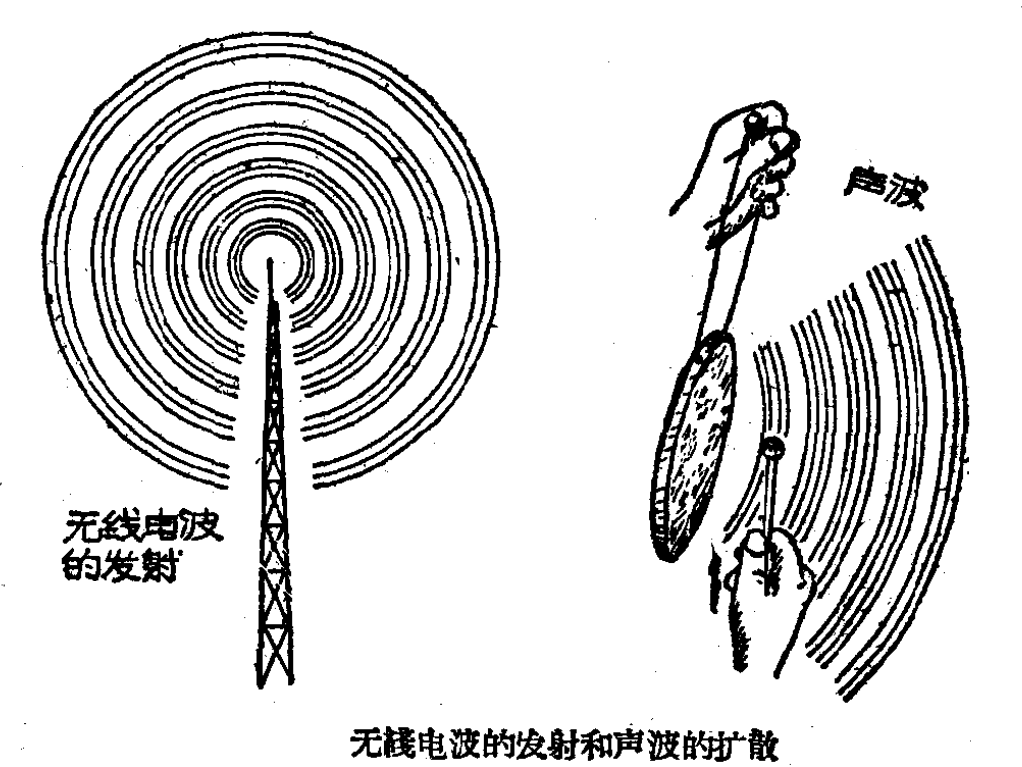
\includegraphics[width=0.7\linewidth]{1}
	\caption{}
	\label{fig:1}
\end{figure}

无线电波虽然漫天遍地都是,但是我们的感觉器官却无法直接感受,无法捕捉。“天线”就是用来捕捉那“来无影去无踪”的无线电波的。打个比方,正好像高挂着的蛛网,又好像昆虫用以探索物体的触须。所以无线电发明者 AC.波波夫就叫它为“Antenna”\footnote{Antenna是从希腊文“触须”一字转借来的,是法国物理学家布隆德尔在波波夫发明天线时写给波波夫信中第一次提出的。},无线电波虽然看不见、嗅不出、摸不着,但它一碰到金属等导电物体就会在这物体中感应出来相应的电压。所以天线是用良导体(如铜线等)做的。

虽然无线电波是无孔不入的,但它也会被高山和高大的建筑物等所阻挡或减弱,所以天线一般都高架在空中。

因此,可以简单地为天线下个定义:“天线\footnote{这里光指收信天线。}是用来捕捉(接收)无线电波的,高张在空中的金属线”。

因为天线是收音机的第一道门户,所以天线的好坏对收音机工作的好坏有非常密切的关系,尤其对比较简单的收音机来说更为重要。例如矿石收音机和单管机,如果没有一根比较好的天线,就不能顺利地收音。

\section{天线的种类}

天线的种类很多,有的以天线外形来分(如T形,Г形等);有的用它的工作原理来分(如行波天线、同相天线等);有用它的工作效能来分的(有定向及非定向等);有以用途来分的。

以用途分大体可分接收天线和发射天线,接收天线就是指用于收音机收报机上的,是用来接收电波的。发射天线是用于发射机的,用以发射电波。

简单的常用接收天线有定向非定向,有T形、Г形、垂直、刷形、环形,有防干扰用的特种天等;其中Г形及T形天线,业余无线电爱好者用得最多。

Г形天线又叫倒L形天线,主要是由水平悬挂的天线和引下接至收音机用的引下线以绝缘子、拉线等附属装置组成。因为它的外形象俄文字母Γ字(或倒的英文字母L)而得名。

\begin{figure}[htbp]
	\centering
	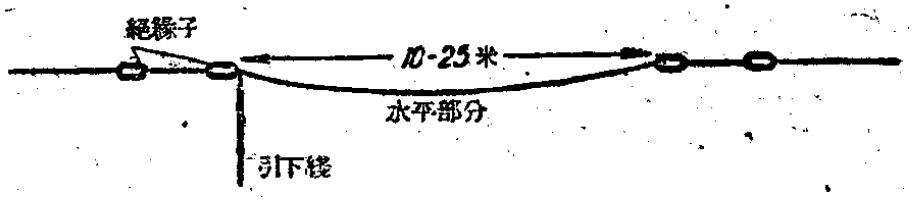
\includegraphics[width=0.7\linewidth]{2}
	\caption{}
	\label{fig:1}
\end{figure}

Γ形天线略有方向性,他接收由引下线一端来的电波的能力最强。但这个性能不很显著,基本上属于非方向性天线。

T形天线和Γ形天线很相像,所不同的是它的引下线不是从天线的一端接出,而是从它的中间接出。这种天线虽然接收来自两头的电波的能力稍强一些,但也不明显,所以也是属于非方向性的。

\begin{figure}[htbp]
	\centering
	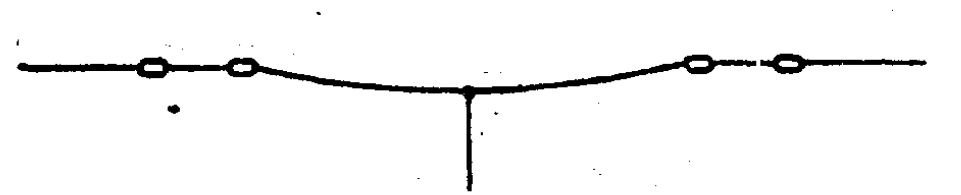
\includegraphics[width=0.7\linewidth]{3}
	\caption{}
	\label{fig:1}
\end{figure}

垂直天线及倾斜天线如下图所示。这两种天线没有水平部分,只有一条重直挂着的或斜挂着的铜线。

\begin{figure}[htbp]
	\centering
	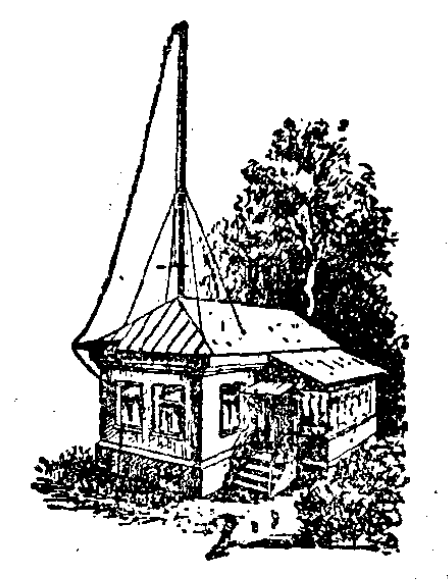
\includegraphics[width=0.7\linewidth]{4}
	\caption{}
	\label{fig:1}
\end{figure}

\begin{figure}[htbp]
	\centering
	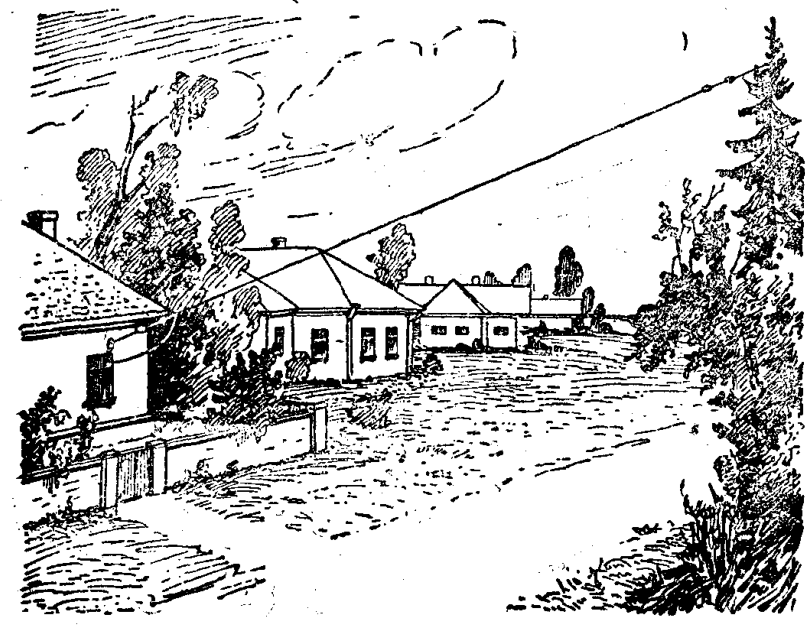
\includegraphics[width=0.7\linewidth]{5}
	\caption{}
	\label{fig:1}
\end{figure}

刷形天线或叫集中电容式天线。它用电容很大的刷状或螺状导线束来代替Г形、T形等的水平部分。

\begin{figure}[htbp]
	\centering
	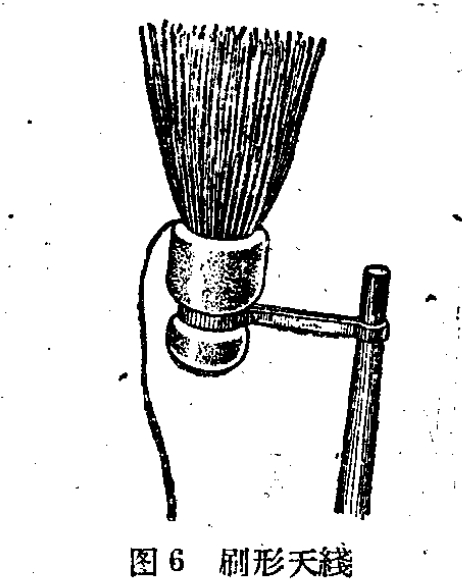
\includegraphics[width=0.7\linewidth]{6}
	\caption{}
	\label{fig:1}
\end{figure}

室内天线及代用天线。最简单的室内天线为一条拖在收音机外面的几尺长的线段,稍考究些的可在天花板下面拉上一段导线,或螺旋形天线。

\begin{figure}[htbp]
	\centering
	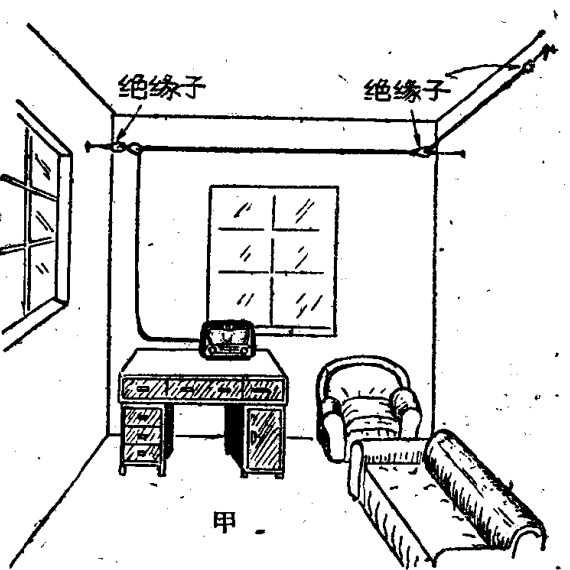
\includegraphics[width=0.7\linewidth]{7}
	\caption{}
	\label{fig:1}
\end{figure}

\begin{figure}[htbp]
	\centering
	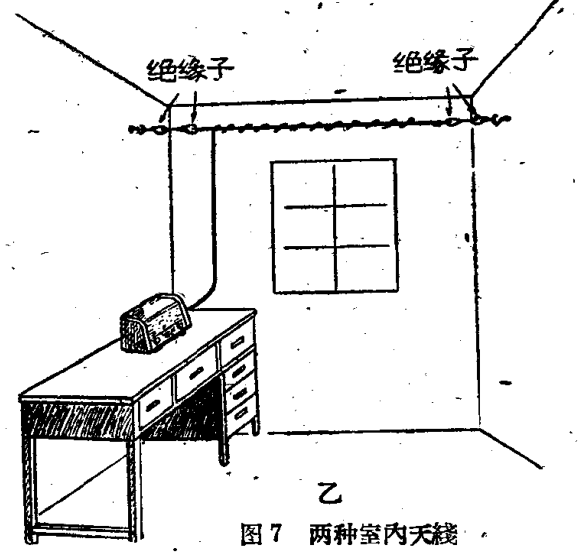
\includegraphics[width=0.7\linewidth]{8}
	\caption{}
	\label{fig:1}
\end{figure}

至于代用天线,它的种类形式就更多了。因为上面已经说过,无线电波不单能在挂着的导线上激起电压(或电流),在一切的导体上都能产生电压。所以如电话机、电灯、铁皮屋顶以至在铁床,铜网纱窗等都可当作代用天线。金属导体的面积愈大,与地的绝缘愈好(对高频电流而言),那么代天线的效果也就愈好。

\section{怎样架设天线}

架设哪一种天线好,这是初学的业余无电爱好者所迫切需要解决的问题,可是对于这问题也很难作出一个“放之四海而皆准”的答复。因为采用那一种天线,要看你所用的收普机和所处的环境来决定。一般来说,装一条Г形天线对于任何收音机都能适用。

\subsection{Γ形天线}

Г形天线是由一根长约10-30米的,高悬着的(约10-20米)多股铜线和引下线组成。当然,单纯从收音的音量强度和收音距离的观点来看,天线愈长愈高,效果也就愈好。但是太长太高了会带来很大的天电干扰、工业干扰及其他妨碍收音的杂音。若附近有大电台时更将会引起夹音,反而不能很好收听。所以天线的长短、高低要看具体环境而定。

一般地说,在附近没有大电台,没有工业干扰(如在村),收音机比较简单,那就应将天线架得长些、高些;若在工业干扰很大、附近电台林立(如在大城市)的地区,天线就应短些、低些。

对一般矿石收音机来说可用长25--30米的天线;二、三管再生式收音机可用15--20米的;超外差收音机可用8--10米,或甚至只用一条几米的短线段。

天线的导线是用由多股0.5--0.7公厘裸线绞合成的2--3公厘的绞合线,或不小于1.5--2公厘的单股铜(16号或14号紫铜线)。不可用黄铜线或铝线,因为它们会很快氧化而变成非常脆弱。在真正没有办法时用1.5--2公厘的镀锌铁线,也可勉强应用。

天线最好是用整条的线,若条件不许可时也可将几段接起来,但必须加以焊接(不要用带酸性的焊剂)。

除导线外,还有一种主要材料是“绝缘子”。绝缘子是不导电的,可以防止天线上的高频电流经杆子等漏入地中。

绝缘子有好多种(可在无线电料商店或电料行中购得),按照制造它们的材料来分,有玻璃的和瓷的,玻璃的比较好,两端孔是穿线用的。瓷绝缘子形如蛋形,故叫蛋形绝缘子,有大有小,收音机天线用直径一寸的就可以了。假如上面两种绝缘子都没有,也可用普通装电灯线的双孔瓷夹板或瓷壶(也叫鼓形白料,)来代替,不得已时也可用玻璃瓶,或甚至用白腊浸煮过的硬木头、纱线圈。

\begin{figure}[htbp]
	\centering
	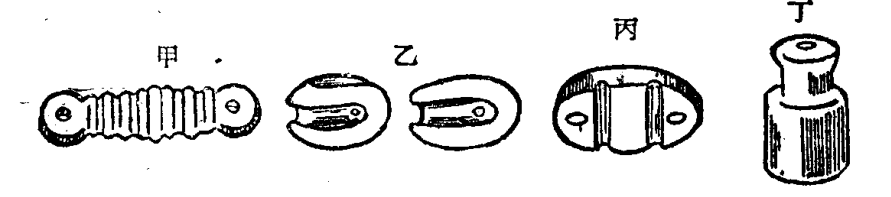
\includegraphics[width=0.7\linewidth]{9}
	\caption{}
	\label{fig:1}
\end{figure}

若引下线要通过墙或窗口,那么还需要几个瓷套管或硬橡胶套管。

\begin{figure}[htbp]
	\centering
	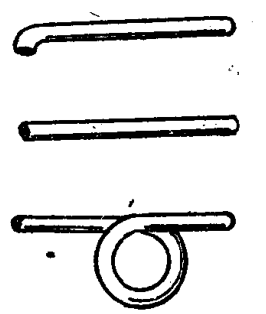
\includegraphics[width=0.7\linewidth]{10}
	\caption{}
	\label{fig:1}
\end{figure}

此外两根高的10-20米的木杆或竹杆,以及若于2.4--4公厘的铁丝(作拉紧天线杆用)和一些螺钉、钉子等,若有一小滑轮就更好了。

在动手架设天线之前必须首先选择好场地。在选择时要考虑到便于利用邻近的房屋、树木等,应尽可能使天线水平部分不跨越屋顶、树木等,使天线水平部分有足够的空间,并且使它尽可能地高些。

其次应法意下列事项:

(1)不使天线和屋篇、墙壁、树木、自来水管、煤气管等相碰

(2)天线不要和电灯线、电话靠得太近或平行,也不要横越这些线上,特别是不要架在高压电力线的上面或下面,因为这样不但容易受到干扰,而且也非常危险。

(3)引人线最好不要贴着墙壁走得太长,也不要拐许多弯,引入线愈短愈好,这样可以减小损失。

为了减短天线杆的长度,可将天线杆固定在屋顶上、大树上或其他高建筑物上。若屋顶上不易装,那么就只好将杆子立在地上了。

为了防止天线上的高频电流经过杆子漏掉,在天线和杆子之间必须要加几个绝缘子,一般每端用两个到三个。它的接法如图。

\begin{figure}[htbp]
	\centering
	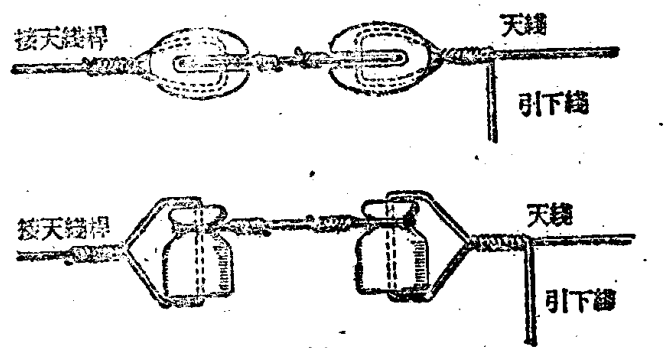
\includegraphics[width=0.7\linewidth]{11}
	\caption{}
	\label{fig:1}
\end{figure}

但不能如下图那样。因为那样接时会使绝缘子受到拉力而破碎。

\begin{figure}[htbp]
	\centering
	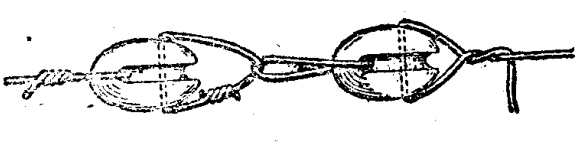
\includegraphics[width=0.7\linewidth]{12}
	\caption{}
	\label{fig:1}
\end{figure}

=====================================================================================================



\section{特种天线}


\chapter{地线}

\section{怎样装地线}

\chapter{矿石收音机}

矿石收音机是一种最简单,最济的收音机,需用器材不多,制作容易,不需要维持费用。这种简单而又经济的收音机,在装置上和检修上都不需要特殊的技术,最合于一般初学的无线电爱好者研究之用。

虽然矿石收音机也有它的缺点,如收程不远,声音小等,但是我国各省现在都已普遍地设立了人民广播电台,故在很大的地区内,矿石收音机仍可使用的。

==============================================================================每一个无电爱好者的研究工作,差不多都是从石收机开始的,本母就是为了具体帮助初学者去制造矿石收音机而寫。里面說明了接收原理;矿石收音机主要零件的 機造 和 性能;收晋机的制作和稚修。采用的零件都是容易贸到或可以自制的,读者只要依酰明安装;就是从來没有学督过无线电的人也能成功。
这是一个无线电爱好者从事制作的开端,在装管碳石收机獲得煦之后,就可以在这个基碰上,选一步去装电学管收管机了。
如果讀者还想在理論方面和制作方面作深一步的研,下面这几本者是比较适合的:
1.'初等电工学
苏联 ·耶列柏卓夫著

\backmatter


矿石收音机 冯报本

无电源收音机	陈鹏飞	黑龙江科学技术出版社 1985	15217.170

\end{document}